\section{Results} \label{sec:results}

To evaluate the performance characteristics of the MCTS dependency calculator, we conducted a sensitivity analysis on the four primary hyperparameters governing the search: Tree Depth (\texttt{MaxDepth}), Computational Budget (\texttt{MaxIterations}), Simulation Horizon (\texttt{MaxSimulationDepth}), and the Exploration Constant ($\lambda$).

\subsection{Experimental Setup}
The evaluation was performed using a set of 12 open-source packages chosen to represent varying degrees of graph complexity, ranging from small utilities to large enterprise frameworks. The test corpus $T$ consists of:
\[
T = \{ \text{axios, express, yargs, webpack, eslint, react-scripts, jest, babel-core, react-dom, vue, next, inquirer} \}
\]
For each package, the calculator was tasked with resolving a valid dependency tree of the peer dependencies since they have to be unique. Regular dependencies are allowed to differ and was intractable for the algorithm. 
We measured the Average Execution Time (ms) against the complexity of the resolution, defined by the number of resolved dependencies.

\subsection{Parameter Sensitivity Analysis}

\subsubsection{Impact of Tree Depth}
Figure \ref{fig:max_depth} illustrates the performance impact of varying the maximum tree depth ($d_{max}$). Counter-intuitively, allowing the search tree to grow deeper ($d_{max}=4$) resulted in significantly lower execution times compared to a shallow tree ($d_{max}=2$).

This phenomenon highlights the efficiency of the MCTS Selection policy (UCT) compared to the random Simulation policy. When $d_{max}$ is low, the algorithm is forced to switch to the stochastic rollout phase early in the resolution process. Since the rollout is heuristic-based and less "intelligent" than the UCT tree search, it requires more attempts to find a valid intersection of constraints. By increasing $d_{max}$ to 4, we allow the "smart" selection phase to resolve more variables, reducing the burden on the simulation phase and leading to faster convergence.

\begin{figure}[htbp]
\centering
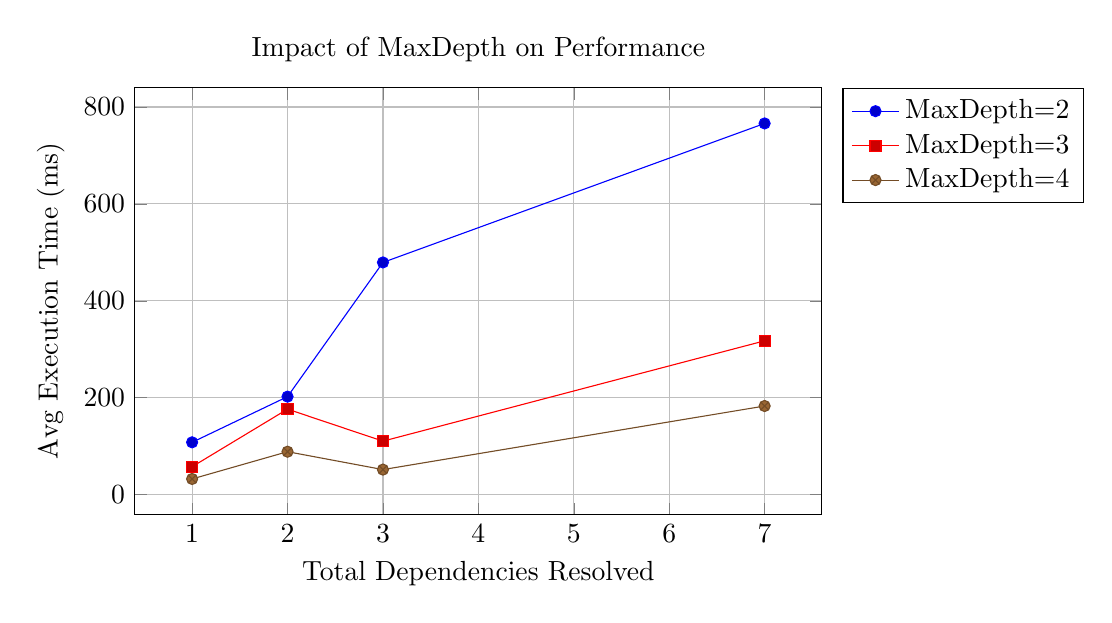
\begin{tikzpicture}
\begin{axis}[
    title={Impact of MaxDepth on Performance},
    xlabel={Total Dependencies Resolved},
    ylabel={Avg Execution Time (ms)},
    grid=major,
    width=0.85\textwidth,
    height=7cm,
    legend pos=outer north east,
    legend cell align={left}
]
\addplot coordinates {(1,108.08) (2,202.32) (3,479.20) (7,766.00) };
\addlegendentry{MaxDepth=2}
\addplot coordinates {(1,57.71) (2,176.55) (3,110.47) (7,317.48) };
\addlegendentry{MaxDepth=3}
\addplot coordinates {(1,32.48) (2,88.72) (3,51.80) (7,183.00) };
\addlegendentry{MaxDepth=4}
\end{axis}
\end{tikzpicture}
\caption{Execution time decreases as Tree Depth increases, indicating that the MCTS tree policy is more efficient than the random rollout.}
\label{fig:max_depth}
\end{figure}

\subsubsection{Impact of Computational Budget}
Figure \ref{fig:max_iterations} confirms the expected linear relationship between the number of MCTS iterations ($k$) and execution time.
\begin{itemize}
    \item At $k=50$, the solver is extremely fast ($<100$ms) but may fail to converge on highly complex graphs like \texttt{react-scripts}.
    \item At $k=1000$, execution time exceeds 1.5 seconds for complex graphs.
\end{itemize}
The data suggests that for interactive applications (e.g., CLI tools), a budget of $k=200$ represents an optimal trade-off, keeping execution time under 400ms while providing sufficient search coverage.

\begin{figure}[htbp]
\centering
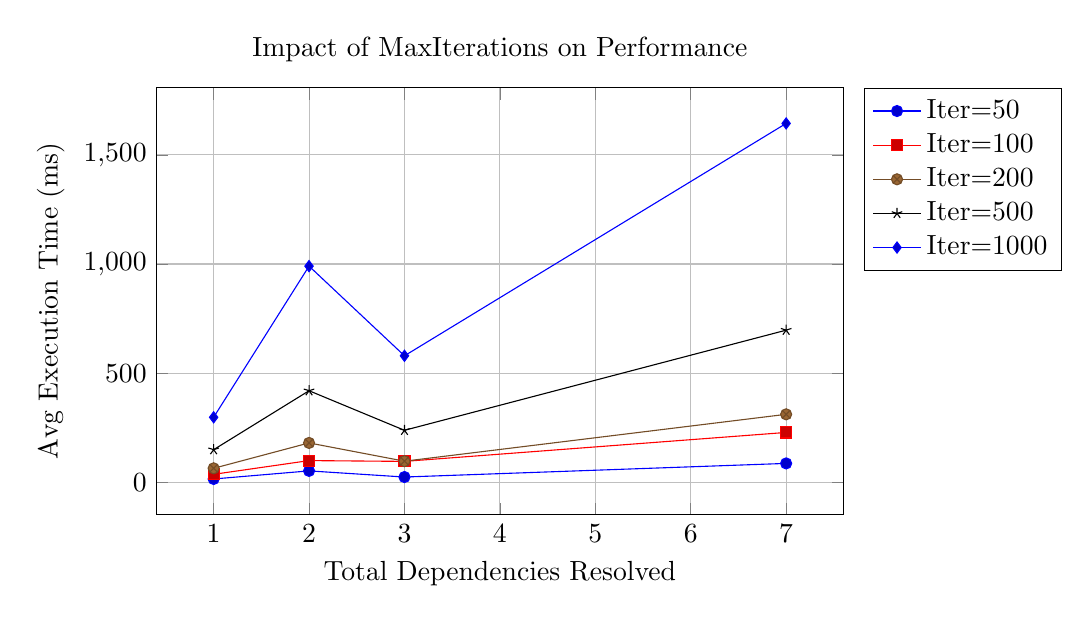
\begin{tikzpicture}
\begin{axis}[
    title={Impact of MaxIterations on Performance},
    xlabel={Total Dependencies Resolved},
    ylabel={Avg Execution Time (ms)},
    grid=major,
    width=0.85\textwidth,
    height=7cm,
    legend pos=outer north east,
    legend cell align={left}
]
\addplot coordinates {(1,15.52) (2,52.56) (3,24.40) (7,86.80) };
\addlegendentry{Iter=50}
\addplot coordinates {(1,36.82) (2,99.71) (3,96.05) (7,228.62) };
\addlegendentry{Iter=100}
\addplot coordinates {(1,64.36) (2,180.60) (3,97.00) (7,311.60) };
\addlegendentry{Iter=200}
\addplot coordinates {(1,149.68) (2,419.64) (3,238.40) (7,697.00) };
\addlegendentry{Iter=500}
\addplot coordinates {(1,297.96) (2,990.32) (3,579.60) (7,1643.80) };
\addlegendentry{Iter=1000}
\end{axis}
\end{tikzpicture}
\caption{Linear scaling of execution time relative to the iteration budget.}
\label{fig:max_iterations}
\end{figure}

\newpage

\subsubsection{Impact of Simulation Horizon}

Figure \ref{fig:sim_depth} analyzes the depth of the rollout phase ($d_{sim}$). We observe a distinct performance cliff. For $d_{sim} \in \{5, 10, 15\}$, performance remains stable and efficient. However, increasing $d_{sim}$ to 50 results in a sharp increase in execution time.
This indicates that the critical constraints in the npm ecosystem are typically local (within 10-15 degrees of separation). Extending the simulation beyond this horizon ($d_{sim}=50$) forces the solver to traverse irrelevant deep dependencies, adding computational overhead without contributing significant information to the Reward function $R$.

\begin{figure}[htbp]
\centering
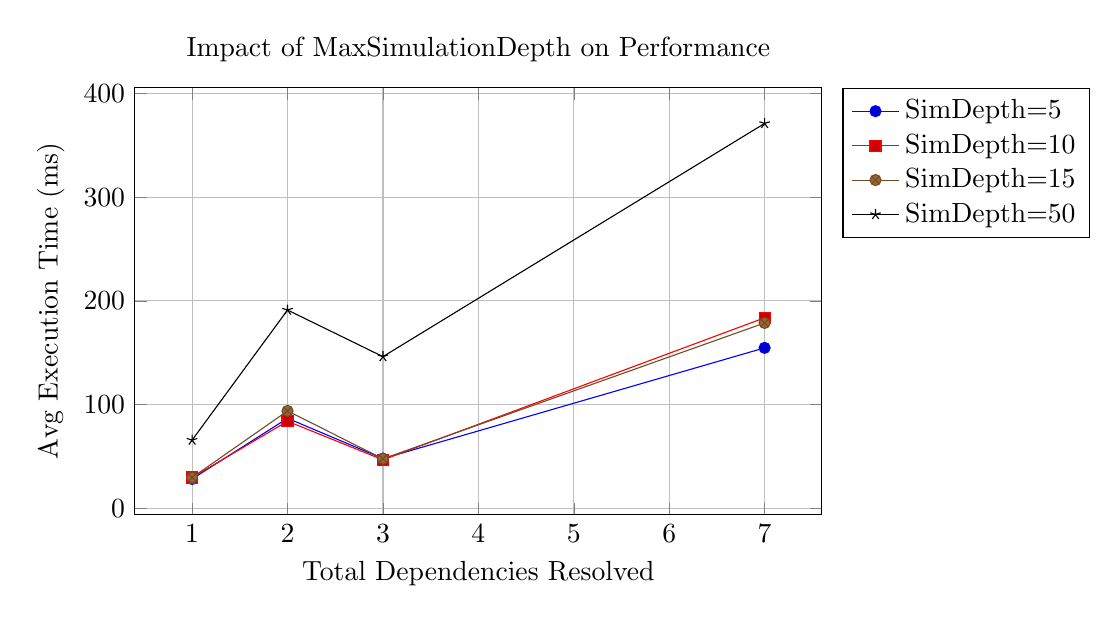
\begin{tikzpicture}
\begin{axis}[
    title={Impact of MaxSimulationDepth on Performance},
    xlabel={Total Dependencies Resolved},
    ylabel={Avg Execution Time (ms)},
    grid=major,
    width=0.85\textwidth,
    height=7cm,
    legend pos=outer north east,
    legend cell align={left}
]
\addplot coordinates {(1,28.16) (2,86.68) (3,47.80) (7,154.60) };
\addlegendentry{SimDepth=5}
\addplot coordinates {(1,29.52) (2,83.84) (3,46.60) (7,183.60) };
\addlegendentry{SimDepth=10}
\addplot coordinates {(1,29.52) (2,93.76) (3,47.60) (7,178.60) };
\addlegendentry{SimDepth=15}
\addplot coordinates {(1,65.64) (2,191.07) (3,146.14) (7,371.03) };
\addlegendentry{SimDepth=50}
\end{axis}
\end{tikzpicture}
\caption{Performance degrades significantly when simulation depth exceeds the effective diameter of the dependency graph.}
\label{fig:sim_depth}
\end{figure}

\subsubsection{Impact of Simulation Bias ($\lambda$)}
Figure \ref{fig:lambda} analyzes the sensitivity of the solver to the weighting parameter $\lambda$ used in the probabilistic rollout \eqref{eq:rollout}. This parameter controls the "greediness" of the heuristic simulation: a low $\lambda$ approaches a uniform random walk, while a high $\lambda$ approaches a deterministic greedy search for the latest version.

The results reveal a non-linear relationship with a distinct performance "sweet spot" at $\lambda = 1.5$:

\begin{itemize}
    \item \textbf{Low Bias ($\lambda=0.5$ - Random):} 
    The solver exhibits poor performance (Avg: 317ms). With a flatter probability distribution, the simulation phase frequently selects older versions during the rollout. This "stale" guidance results in low recency rewards ($R$), providing a weak gradient for the MCTS backpropagation to identify the optimal path.

    \item \textbf{High Bias ($\lambda \geq 3.0$ - Greedy):} 
    Performance recovers and becomes efficient ($\approx 145$ms). For the majority of the test corpus (standard healthy packages), the latest versions are valid. A high $\lambda$ forces the simulation to immediately verify the "latest" path. If valid, it returns a high reward ($R \approx 1.0$) quickly. However, this setting is risky for complex conflict scenarios, as the lack of randomness prevents the simulation from stumbling upon valid older versions.

    \item \textbf{Optimal Balance ($\lambda = 1.5$):} 
    The fastest execution times ($\approx 140$ms) are observed here. This setting provides strong heuristic guidance (favoring new versions) while retaining sufficient entropy to explore alternative version combinations when the latest versions induce a conflict.

    \item \textbf{Transition Instability ($\lambda = 2.0$):} 
    A notable performance degradation (spike to 392ms) occurs at $\lambda = 2.0$. We hypothesize this represents a region of probabilistic interference where the distribution is neither random enough to bypass conflicts easily nor greedy enough to force a rapid (but potentially failed) conclusion, causing the solver to thrash between suboptimal branches.
\end{itemize}

\begin{figure}[htbp]
\centering
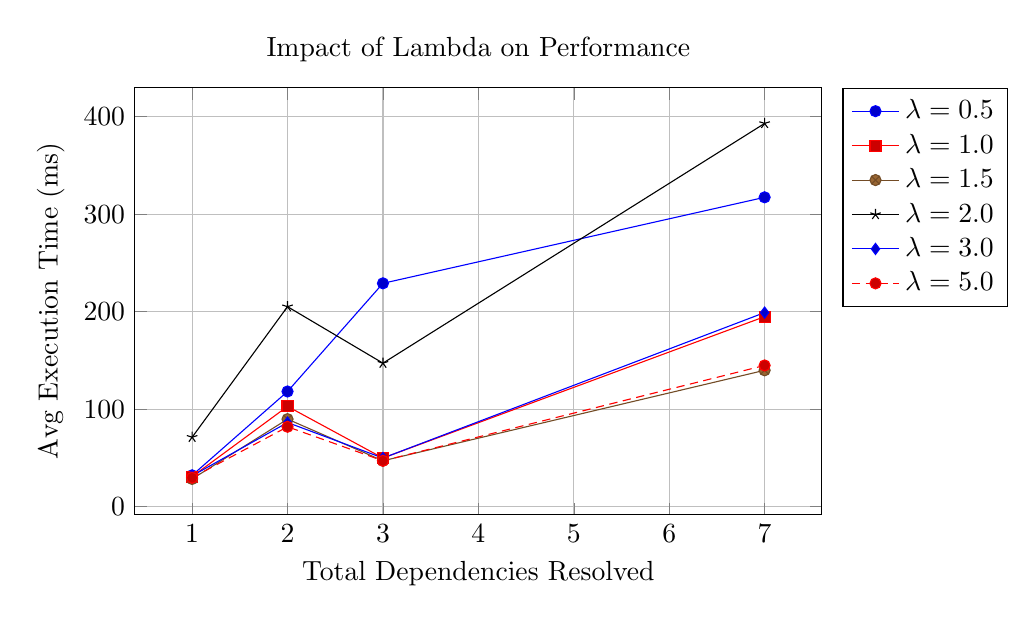
\begin{tikzpicture}
\begin{axis}[
    title={Impact of Lambda on Performance},
    xlabel={Total Dependencies Resolved},
    ylabel={Avg Execution Time (ms)},
    grid=major,
    width=0.85\textwidth,
    height=7cm,
    legend pos=outer north east,
    legend cell align={left}
]
\addplot coordinates {(1,32.08) (2,118.08) (3,229.00) (7,317.20) };
\addlegendentry{$\lambda=0.5$}
\addplot coordinates {(1,30.76) (2,102.80) (3,49.80) (7,194.80) };
\addlegendentry{$\lambda=1.0$}
\addplot coordinates {(1,28.36) (2,89.72) (3,47.00) (7,139.80) };
\addlegendentry{$\lambda=1.5$}
\addplot coordinates {(1,71.15) (2,205.05) (3,147.12) (7,392.97) };
\addlegendentry{$\lambda=2.0$}
\addplot coordinates {(1,31.56) (2,86.24) (3,49.80) (7,199.00) };
\addlegendentry{$\lambda=3.0$}
\addplot coordinates {(1,29.64) (2,81.88) (3,47.00) (7,144.80) };
\addlegendentry{$\lambda=5.0$}
\end{axis}
\end{tikzpicture}
\caption{Exploration parameter tuning. $\lambda=1.5$ provides the optimal balance, while deviations lead to increased search times.}
\label{fig:lambda}
\end{figure}

\clearpage